%\title{Title page with logo}
%----------------------------------------------------------------------------------------
%	PACKAGES AND OTHER DOCUMENT CONFIGURATIONS
%----------------------------------------------------------------------------------------

\documentclass[12pt]{article}
\usepackage[portuges]{babel}
\usepackage[utf8]{inputenc}
\usepackage[hyphens]{url}
\usepackage{graphicx}
\usepackage[hidelinks]{hyperref}
\usepackage[toc,page]{appendix}
\usepackage{indentfirst}
\usepackage[table,xcdraw]{xcolor}
\usepackage{longtable}
\usepackage[margin=4cm]{geometry}

\newcommand{\tabitem}{~~\llap{\textbullet}~~}

\renewcommand\appendixtocname{Anexos}
\renewcommand\appendixpagename{Anexos}

\begin{document}
\sloppy
\LTcapwidth=\textwidth

\begin{titlepage}

\newcommand{\HRule}{\rule{\linewidth}{0.5mm}} % Defines a new command for the horizontal lines, change thickness here

\center % Center everything on the page

\vspace{0.5cm}
 
%----------------------------------------------------------------------------------------
%	HEADING SECTIONS
%----------------------------------------------------------------------------------------

\textsc{\LARGE Scripting no Processamento}\\[0.3cm]
\textsc{\LARGE de Linguagem Natural}\\[1.1cm] % Name of your university/college
\textsc{\Large Universidade do Minho}\\[0.5cm] % Major heading such as course name
\textsc{\large Mestrado Integrado em Engenharia Informática}\\[0.5cm] % Minor heading such as course title

%----------------------------------------------------------------------------------------
%	TITLE SECTION
%----------------------------------------------------------------------------------------
\vspace{0.8cm}
\HRule \\[0.6cm]
{ \huge \bfseries Trabalho Prático 2}\\[0.4cm] % Title of your document
{ \Large \bfseries spaCy's POS Tagging}\\[0.4cm] % Subtitle of your document
\HRule \\[1.0cm]
 
%----------------------------------------------------------------------------------------
%	AUTHOR SECTION
%----------------------------------------------------------------------------------------

\Large \emph{Grupo 7:}\\
A73831 - João Miguel Pires Barreira\\
A77364 - Mafalda Nunes\\[1.3cm]

%----------------------------------------------------------------------------------------
%	DATE SECTION
%----------------------------------------------------------------------------------------

{\large \today}\\[1.5cm] % Date, change the \today to a set date if you want to be precise

%----------------------------------------------------------------------------------------
%	LOGO SECTION
%----------------------------------------------------------------------------------------


\includegraphics[width=0.55\textwidth]{logo}\\[1cm] % Include a department/university logo - this will require the graphicx package
 
%----------------------------------------------------------------------------------------

\vfill % Fill the rest of the page with whitespace

\end{titlepage}

\vspace{0.5cm}

\begin{abstract}
O presente relatório tem com objetivo a aprendizagem das funcionalidades da ferramenta \textit{spaCy}. Para tal, apresentar-se-á uma descrição da mesma, mais especificamente da
funcionalidade de POS \textit{tagging}, bem como um pequeno exemplo que demonstre como utilizar a ferramenta.

Este trabalho pretende dar resposta ao trabalho prático 2, proposto na unidade curricular SPLN, do Mestrado em Engenharia Informática, da Universidade do Minho.
\end{abstract}

\vspace{0.5cm}

\tableofcontents

\newpage

\let\oldref\ref
\renewcommand{\ref}[1]{\smash{\underline{\oldref{#1}}}}

\section{spaCy's}

spaCy é uma biblioteca \textit{open-source} para o processamento de linguagem natural em \textit{Python}. É uma aplicação desenvolvida especificamente para o uso em ambientes de 
produção, que não só processa mas também ajuda a "compreender" grandes volumes de texto. Dentro deste contexto, pode ser utilizada em muitas vertentes, desde a extração de
conhecimento, obtenção de conhecimento léxico sobre linguagens, ou pré-processamento de texto para \textit{deep-learning}.

% Falar sobre o que é
% https://spacy.io/usage/spacy-101
% https://spacy.io/usage/v2

\subsection{Arquitetura} % Mafalda

% https://spacy.io/api/

\subsection{Funcionalidades}

\begin{itemize}
	\item \textbf{Tokenization} -- Separação de textos em segmentos significativos, como palavras, pontuação,  entre outros. Esta divisão é efetuada tendo em conta regras
								   específicas de cada linguagem. O \textit{input} corresponde a um texto limpo e o \textit{output} um objeto \textit{Doc}.
	\item \textbf{Part-of-speech (POS) Tagging} -- 
	\item \textbf{Dependency Parsing} -- Processo de obtenção de relações de dependência entre os elementos de uma frase através de um \textit{parser}. Este \textit{parser}
										 possibilita a iteração do texto \textit{tokenizado} (\textit{Doc}) pelas suas frases nominais, sendo que as dependências são dispostas numa
										 árvore de fácil manipulação. É ainda possível visualizar mais facilmente as dependências de um ou mais \textit{Docs} através de um grafo,
										 cujos arcos possuem uma legenda que caracteriza a ligação sintática entre os \textit{tokens}.
	\item \textbf{Lemmatization} --
	\item \textbf{Sentence Boundary Detection (SBD)} -- Processo de separação de frases de um texto separado pelos seus \textit{tokens} (\textit{Doc}). É utilizado o \textit{parsing}
														de dependências para uma divisão mais correta. Possibilita a definição manual dos limites frásicos (i.e. \textit{boundaries})
														em detrimento dos pré-definidos '.', '!' e '?'.
	\item \textbf{Named Entity Recognition (NER)} --
	\item \textbf{Similarity} -- Comparação de dois textos e cálculo de valor que indique quão similares são. A função de similitude compara palavras de um dado texto com base em
								 vetores de palavras específicos para cada linguagem que podem ser customizados para um melhor desempenho em contextos de aplicação específicos.
	\item \textbf{Text Classification} -- 
	\item \textbf{Rule-based matching} -- Processo de busca de correspondências entre \textit{tokens} e determinados padrões. Estes padrões podem ser bastante complexos, tendo
										  algumas parecenças com o funcionamento expressões regulares. No entanto, podem também tirar partido do conhecimento léxico desta ferramenta,
										  filtrando, por exemplo, por bases morfológicas (i.e. \textit{Lemma}) ou classes gramaticais (i.e. verbos, substantivos, etc.). Possibilita
										  ainda a formulação de padrões mais complexos através de quantificadores, \textit{wildcards}, expressões regulares. Podem ainda ser definidas,
										  de um modo simples, funções que serão chamadas caso se dê uma ou mais correspondências.
	\item \textbf{Training} --
	\item \textbf{Serialization} -- Funcionalidade responsável por guardar objetos do \textit{spaCy} para ficheiros em disco, bem como por carregar objetos previamente guardados. Este
									processo torna-se especialmente importante quando usado para guardar objetos do tipo \textit{Doc}, por exemplo, que possuem todas as informações
									retiradas do texto original, bem como outras características inseridas manualmente como entidades ou vetores de palavras customizados. Para isso, é
									utilizado  a biblioteca \textit{Pickle}, \textit{built-in} da linguagem \textit{Python}.
\end{itemize}

% Falar de forma relativamente geral, mas com imagens para se perceber (informação de POS tagging pode ser aprofundada e utilizada na próxima secção)

% fala um bocadinho mais de reconhecimento de entidades e grafos de dependencias

% https://spacy.io/usage/spacy-101
% https://spacy.io/usage/linguistic-features
% https://spacy.io/usage/processing-pipelines
% https://spacy.io/usage/vectors-similarity
% https://spacy.io/usage/training
% https://spacy.io/usage/adding-languages
% https://spacy.io/usage/visualizers

% https://spacy.io/usage/v2
% https://spacy.io/api/annotation
% https://spacy.io/api/top-level

% https://towardsdatascience.com/a-short-introduction-to-nlp-in-python-with-spacy-d0aa819af3ad
% https://towardsdatascience.com/a-review-of-named-entity-recognition-ner-using-automatic-summarization-of-resumes-5248a75de175


\subsection{Vantagens} % Mafalda

% https://spacy.io/usage/facts-figures
% https://www.analyticsvidhya.com/blog/2017/04/natural-language-processing-made-easy-using-spacy-%E2%80%8Bin-python/
% https://medium.com/@brianray_7981/ai-in-practice-identifying-parts-of-speech-in-python-8a690c7a1a08

\subsection{Utilização} % João

O processo de instalação da biblioteca é bastante simples, podendo ser realizado através do \textit{pip} (\textit{package manager} da linguagem \textit{Python}), utilizado, neste
exemplo, na sua versão 3.X.

\begin{verbatim}
	$ pip3 install spacy
\end{verbatim}

Os modelos correspondentes às linguagens podem ser também facilmente obtidos através do seguinte comando abaixo, exemplificado para um dos modelos da língua inglesa.

\begin{verbatim}
	$ python3 -m spacy download en_core_web_sm
\end{verbatim}

Após o processo de instalação da biblioteca e de \textit{download} das linguagens, o primeiro passo será importar a biblioteca. Depois, poder-se-á carregar a linguagem já
descarregada e produzir um \textit{Doc} a partir de um qualquer texto. Será então possível começar imediatamente a tirar proveito das funcionalidades providenciadas pela biblioteca,
utilizando o objeto do tipo \textit{Doc} resultante do processamento do texto inserido.

\begin{verbatim}
	>>> import spacy
	>>> nlp = spacy.load('en_core_web_sm')
	>>> doc = nlp('This text can now be processed using spaCy!')
\end{verbatim}

% https://spacy.io/api/cli
% https://spacy.io/usage/

\subsection{Aplicações}

% https://spacy.io/usage/examples
% https://github.com/explosion/spacy/blob/master/examples/information_extraction/entity_relations.py

% grafos de dependencias Mafalda
% reconhecimento de entidades João
% exceção de tokens Mafalda
% exemplos da net João

\subsubsection{Grafos de dependências}
\subsubsection{Reconhecimento de entidades}

Dentro do âmbito deste trabalho prático o grupo desenvolveu um reconhecedor de entidades. Esta ferramenta efetua o reconhecimento de entidades de um texto dado como \textit{input}
tanto para o terminal, como para um ficheiro de \textit{output}. A figura seguinte mostra o exemplo do output gerado para o terminal.

\begin{figure}[!ht]
	\centering
	\makebox[\textwidth][c]{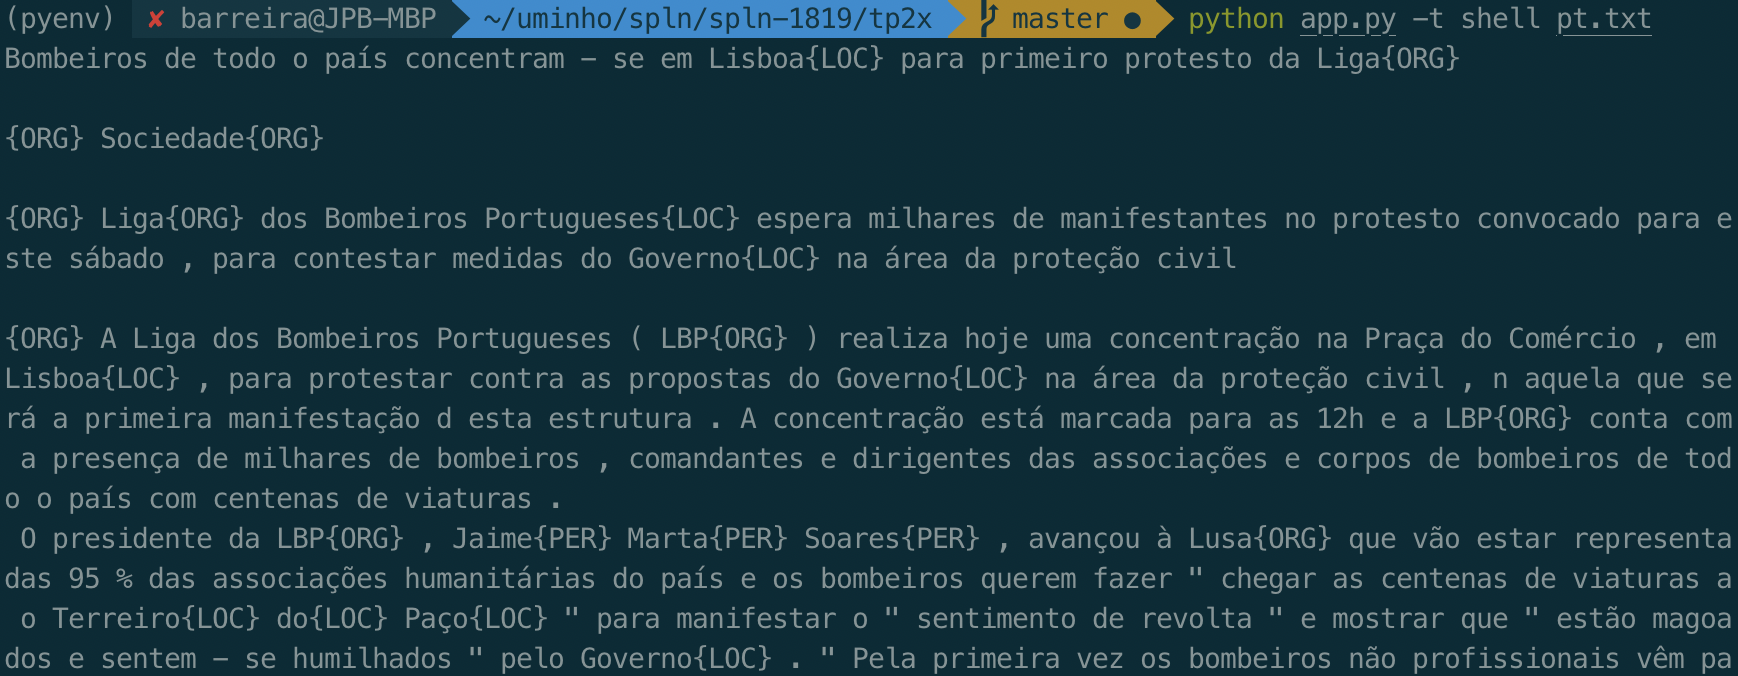
\includegraphics[width=10cm]{shell.png}}
	\caption{Reconhecimento de entidades num texto em português (shell)}
\end{figure}

\newpage
Adicionalmente, no contexto da aplicação \textit{web} também desenvolvida, é ainda possível ser gerado código \textit{HTML} que permite a uma visualização mais simples e intuitiva do
resultado final, como mostra a figura abaixo.

\begin{figure}[!ht]
	\centering
	\makebox[\textwidth][c]{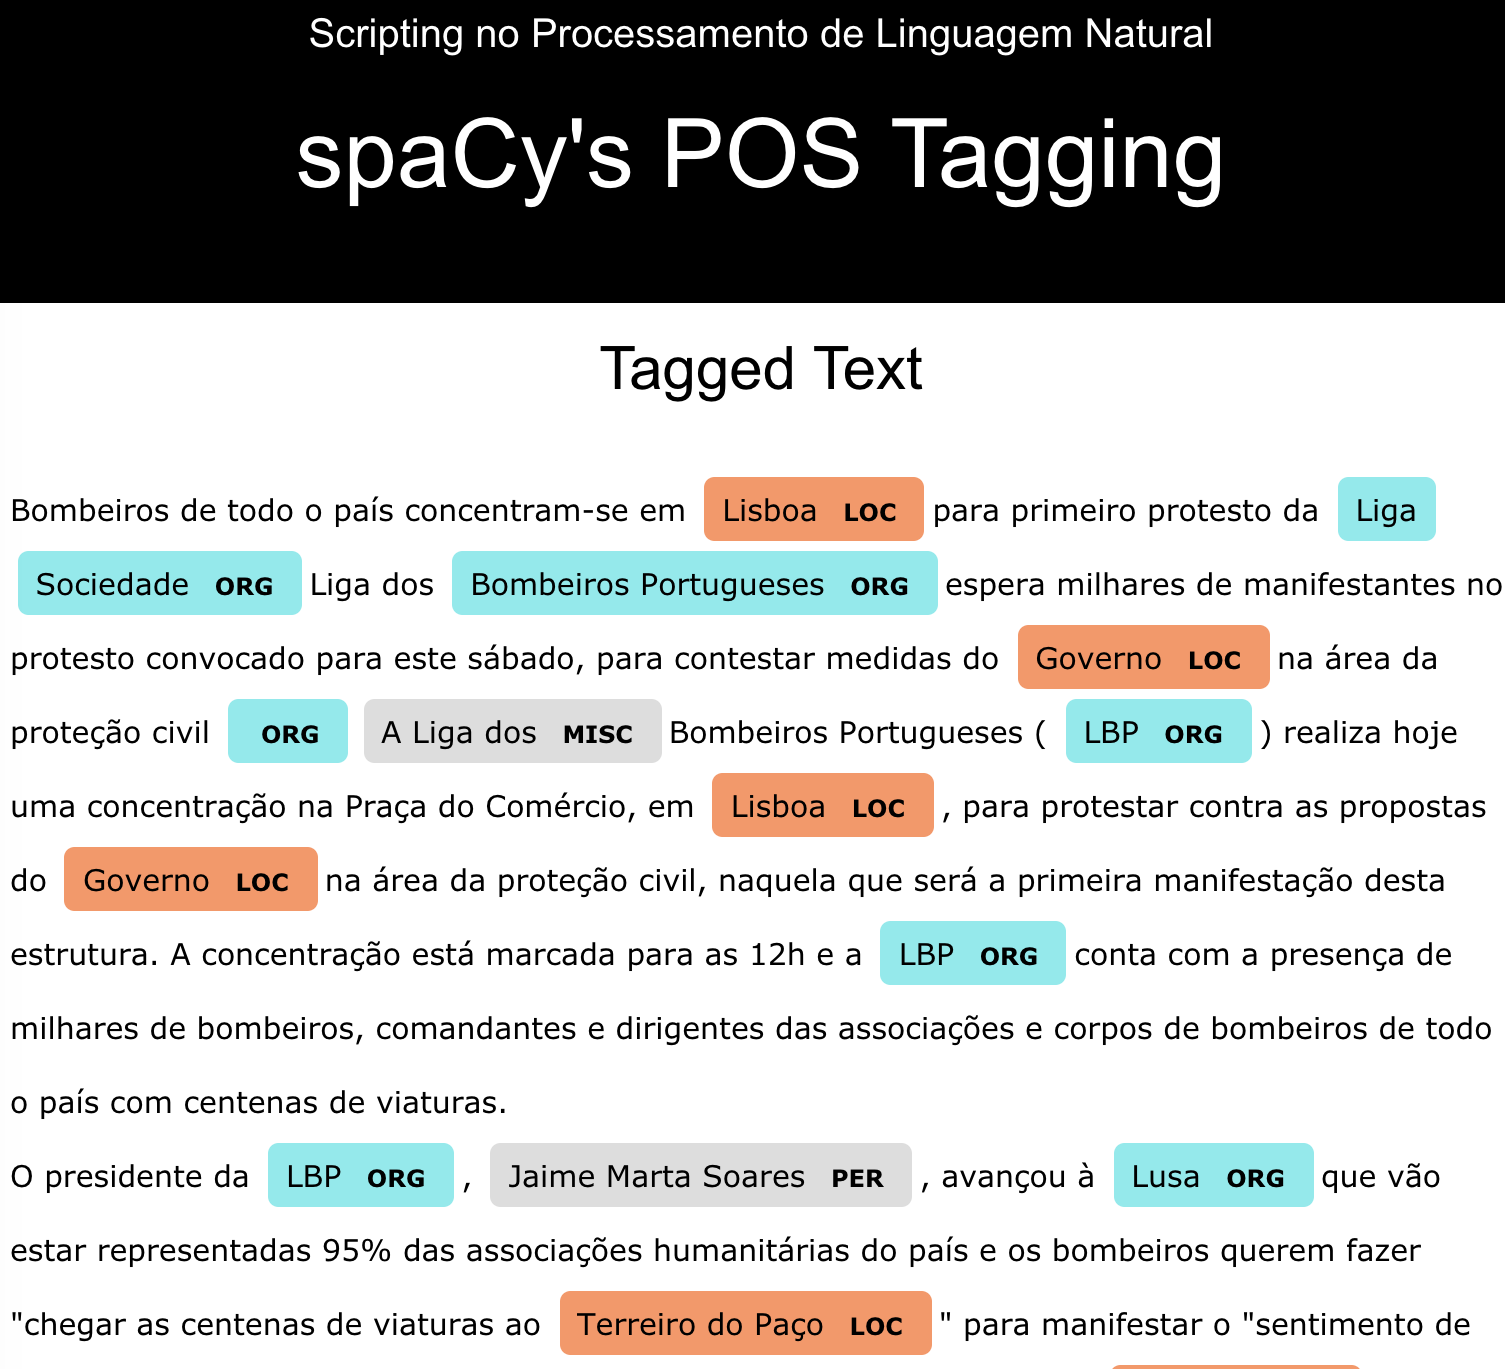
\includegraphics[width=10cm]{ent.png}}
	\caption{Reconhecimento de entidades num texto em português (html)}
\end{figure}

No ambiente \textit{web} é ainda possível fazer uma filtragem dos tipos de entidades que serão tratados, como mostra a figura seguinte.

\begin{figure}[!ht]
	\centering
	\makebox[\textwidth][c]{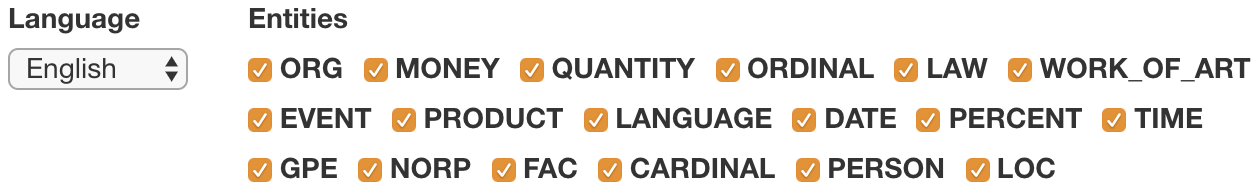
\includegraphics[width=10cm]{filter.png}}
	\caption{Filtragem de tipos de entidades para a língua inglesa }
\end{figure}

O código da função que implementa ambas estas funcionalidades (\textit{web} e \textit{shell}/ficheiro), encontra-se no Anexo B. Antes de ser chamada, é carregada a linguagem
escolhida (ou a por defeito, \textit{pt}) e processado o texto de input. Depois, a função em anexo é chamada com o tipo 'text' para a vertente \textit{shell}/ficheiro, ou
\textit{'html'} para ser apresentado o resultado no contexto da aplicação \textit{web}.

De seguida -- para o caso  \textit{'text'} --, são iteradas as palavras do objeto \textit{Doc}. Caso uma palavra seja reconhecida como pertencendo a um tipo de entidades, é marcada
com o nome do respetivo tipo de entidades a que pertence entre chavetas.

O caso do tipo \textit{'html'} é de implementação bastante simples, visto que se recorre à função \textit{displacy.render} -- pertencente à \textit{API} dos \textit{visualizers} do
\textit{spaCy} --, para gerar o \textit{output} gráfico do reconhecedor de imagens. Este código \textit{HTML} é depois integrado no contexto da nossa aplicação \textit{web}.

\subsubsection{Exceção de tokens}
\subsubsection{Treino do dependency parser}

Como foi dito anteriormente, o \textit{spaCy} possibilita o treino de novos modelos estatísticos utilizados nas suas mais diversas funcionalidades. Umas dessas funcionalidades --
demonstrada neste exemplo --, é o \textit{dependency parser}.

Em primeiro lugar, é criada uma variável \textit{TRAIN\_DATA} que possui duas frases nominais, bem como o nome das dependências (\textit{deps}) e quais os elementos principais dessas
mesmas dependências (\textit{heads}). Esta variável servirá como base para o processo de treino. De seguida, é criada a linguagem que poderá ser uma das pré-existentes, ou criada de
raíz (i.e. \textit{blank}). Depois, é adicionado o \textit{parser} à \textit{pipeline} e adicionadas as etiquetas com os nomes das dependências ao \textit{parser} que é finalmente
utilizado para treinar a linguagem utilizando a variável \textit{TRAIN\_DATA} criada anteriormente. O resultado é, a seguir,
testado, através da impressão do resultado das dependências para um novo texto.

Adicionalmente, tira-se ainda partido da capacidade de serialização do \textit{spaCy} (abordada anteriormente neste relatório) para guardar o modelo da linguagem que se encontra
modificada após o processo de treino.

O código deste exemplo está presente no Anexo D, encontrando-se também disponível no repositório do \textit{GitHub} (link: X).

\section{spaCy's POS Tagging} % Mafalda

% Aprofundar tema usando websites relevantes indicados nas funcionalidades

\subsection{Utilização} % João

Após ter sido instalada a biblioteca e feito o \textit{download} das linguagens (processo descrito anteriormente), poder-se-á testar o processo de obtenção das \textit{POS tags} para
um determinado texto, de forma simples. Para tal, bastará introduzir um texto de input e -- como apresenta o código abaixo --, imprimir, por exemplo, a informação sobre as
\textit{POS tags} de cada uma das suas palavras.

\begin{verbatim}
	>>> import spacy
	>>> nlp = spacy.load('en_core_web_sm')
	>>> doc = nlp('This is a demonstration of a very cool Python library!')
	>>> for token in doc:
	...    print(token.text, token.pos_)
	This DET
	is VERB
	a DET
	demonstration NOUN
	of ADP
	a DET
	very ADV
	cool ADJ
	Python PROPN
	library NOUN
	! PUNCT	
\end{verbatim}

\section{Exemplo Demonstrativo} % Mafalda

% Falar das funções que desenvolvemos

% Implementar?
% https://books.google.pt/books?id=48RiDwAAQBAJ&pg=PA80&lpg=PA80&dq=spacy+attrs&source=bl&ots=R2y5H5s6e5&sig=33zo94rAGOHBR5PxOH51J1GrBGM&hl=pt-PT&sa=X&ved=2ahUKEwiNlpbKoO_eAhWmJcAKHetlCfQ4ChDoATAAegQICRAB#v=onepage&q=spacy%20attrs&f=false




% Anexos

\setcounter{section}{0}
\setcounter{subsection}{0}


\newpage

\appendixpage
\renewcommand{\thesubsection}{\Alph{subsection}}

\subsection{Exemplo de aplicação: Grafos de dependências}
\label{anexo:dependencias}

\begin{verbatim}
	
\end{verbatim}

\subsection{Exemplo de aplicação: Reconhecimento de entidades}
\label{anexo:reconhecimento}

\begin{verbatim}
	# Visualizing the entity recognizer
	def generate_tagged_text(doc, type = 'server', entities = None, colors = None):
		res = ''
		if type in ('server', 'html'):
			options = {}
			if entities:
				options['ents'] = entities
			if colors:
				options['colors'] = colors
			if type=='server':
				displacy.serve(doc, style='ent', options=options)
			else:
				res = displacy.render(doc, style='ent', options=options)
		else:
			res_list = []
			for word in doc:
				if word.ent_type_:
					res_list.append(str(word) + '{' + word.ent_type_ + '}')
				else:
					res_list.append(str(word))
			res = ' '.join(res_list)
		return res
\end{verbatim}

\subsection{Exemplo de aplicação: Exceção de \textit{tokens}}
\label{anexo:tokens}

\begin{verbatim}
	
\end{verbatim}

\subsection{Exemplo de aplicação: Treino do \textit{dependency parser} (e serialização)}
\label{anexo:treino}

\begin{verbatim}
	#!/usr/bin/env python

	# https://spacy.io/usage/examples#parser

	from __future__ import unicode_literals, print_function

	import plac
	import random
	from pathlib import Path
	import spacy
	from spacy.util import minibatch, compounding


	# training data
	TRAIN_DATA = [
		("They trade mortgage-backed securities.", {
			'heads': [1, 1, 4, 4, 5, 1, 1],
			'deps': ['nsubj', 'ROOT', 'compound', 'punct', 'nmod', 'dobj', 'punct']
		}),
		("I like London and Berlin.", {
			'heads': [1, 1, 1, 2, 2, 1],
			'deps': ['nsubj', 'ROOT', 'dobj', 'cc', 'conj', 'punct']
		})
	]


	@plac.annotations(
		model=("Model name. Defaults to blank 'en' model.", "option", "m", str),
		output_dir=("Optional output directory", "option", "o", Path),
		n_iter=("Number of training iterations", "option", "n", int))
	def main(model=None, output_dir=None, n_iter=10):
		"""Load the model, set up the pipeline and train the parser."""
		if model is not None:
			nlp = spacy.load(model)  # load existing spaCy model
			print("Loaded model '%s'" % model)
		else:
			nlp = spacy.blank('en')  # create blank Language class
			print("Created blank 'en' model")

		# add the parser to the pipeline if it doesn't exist
		# nlp.create_pipe works for built-ins that are registered with spaCy
		if 'parser' not in nlp.pipe_names:
			parser = nlp.create_pipe('parser')
			nlp.add_pipe(parser, first=True)
		# otherwise, get it, so we can add labels to it
		else:
			parser = nlp.get_pipe('parser')

		# add labels to the parser
		for _, annotations in TRAIN_DATA:
			for dep in annotations.get('deps', []):
				parser.add_label(dep)

		# get names of other pipes to disable them during training
		other_pipes = [pipe for pipe in nlp.pipe_names if pipe != 'parser']
		with nlp.disable_pipes(*other_pipes):  # only train parser
			optimizer = nlp.begin_training()
			for itn in range(n_iter):
				random.shuffle(TRAIN_DATA)
				losses = {}
				# batch up the examples using spaCy's minibatch
				batches = minibatch(TRAIN_DATA, size=compounding(4., 32., 1.001))
				for batch in batches:
					texts, annotations = zip(*batch)
					nlp.update(texts, annotations, sgd=optimizer, losses=losses)
				print('Losses', losses)

		# test the trained model
		test_text = "I like securities."
		doc = nlp(test_text)
		print('Dependencies', [(t.text, t.dep_, t.head.text) for t in doc])

		# save model to output directory
		if output_dir is not None:
			output_dir = Path(output_dir)
			if not output_dir.exists():
				output_dir.mkdir()
			nlp.to_disk(output_dir)
			print("Saved model to", output_dir)

			# test the saved model
			print("Loading from", output_dir)
			nlp2 = spacy.load(output_dir)
			doc = nlp2(test_text)
			print('Dependencies', [(t.text, t.dep_, t.head.text) for t in doc])


	if __name__ == '__main__':
		plac.call(main)

		# expected result:
		# [
		#   ('I', 'nsubj', 'like'),
		#   ('like', 'ROOT', 'like'),
		#   ('securities', 'dobj', 'like'),
		#   ('.', 'punct', 'like')
		# ]
\end{verbatim}

%\subsection{Título}
%\label{anexo:nome}
%\begin{figure}[!ht]
%	\centering
%	\makebox[\textwidth][c]{\includegraphics[width=13cm]{Pictures/...}}
%	\caption{Legenda}
%\end{figure}

\newpage

\begin{thebibliography}{99}
	
	\bibitem{linkname}
	Autor,
	``Título'',
	\textit{website name},
	\url{website link}.
	
\end{thebibliography}

\end{document}